

\section{Questão 7}


\subsubsection{Considere a trama de dados nº431. Sabendo que o campo \textit{Frame Control} contido no cabeçalho das tramas 802.11 permite especificar a direccionalidade das tramas, o que pode concluir face à direccionalidade dessa trama, será local à WLAN?}

    \par Ao analisarmos a trama, mais especificamente o campo \textit{Frame Control}, conseguimos denotar o valor das \textit{flags} do mesmo. Para a pergunta em questão, a \textit{flag} que procuramos é a \textbf{DS \textit{status}}, tendo esta dois valores a preencher: \textit{To} DS/AP (destino no AP) e \textit{From} DS/AP (origem no AP). De acordo com a trama, os valores de \textit{To} DS e \textit{From} DS são, respetivamente, \textbf{0} e \textbf{1}, ou seja, estamos perante uma trama que foi enviada através de um AP para um STA, podendo concluir que a trama é local à WLAN.

    \begin{figure}[H]
    \centering
    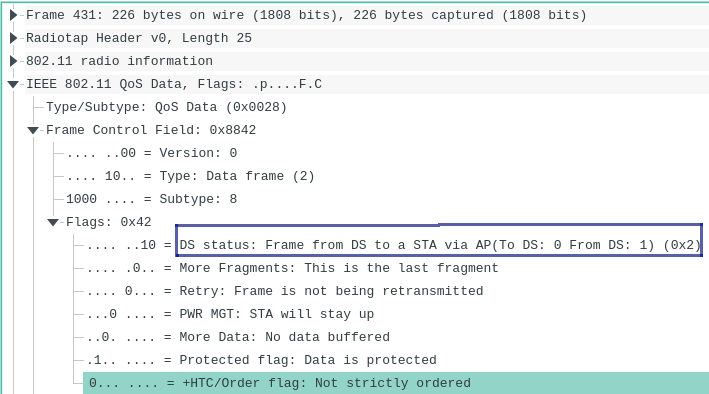
\includegraphics[width=400pt]{Prints/Questao7/questao7-A.png}
    \caption{Captura da Trama Nº 431.} \label{questao7-1-trama431}
    \end{figure}





\vspace{20pt}
\subsubsection{Para a trama de dados nº431, transcreva os endereços MAC em uso, identificando qual o endereço MAC correspondente ao host sem fios (STA), ao AP e ao \textit{router} de acesso ao sistema de distribuição?}

    \par Para além da análise da trama, utilizamos a funcionalidade \textit{hexdump} do \textit{Wireshark}, tendo assim acesso aos \textit{bytes} ordenados da trama. Como tal, conseguimos distinguir três endereços: \textit{receiver} (\textbf{64:9a:be:10:6a:f5}), \textit{transmitter} (\textbf{bc:14:01:af:b1:98}) e \textit{router interface} (\textbf{bc:14:01:af:b1:98}).

    \par Como podemos verificar, o endereço do \textit{host} sem fios (STA) corresponde ao endereço do \textit{receiver}, logo esta trama tem como destino o mesmo. Relativamente aos endereços do AP e do \textit{router}, estes são idênticos, o que nos leva a concluir que o AP realiza tanto as funcionalidades de \textit{routing} como de transmissão de tramas.
    
    \begin{figure}[H]
    \centering
    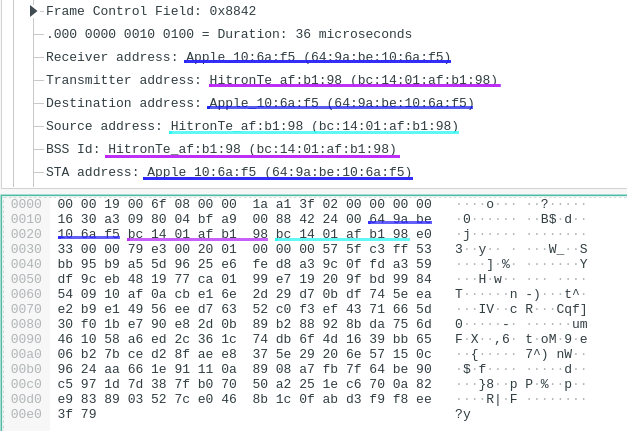
\includegraphics[width=350pt]{Prints/Questao7/questao7-B-1.png}
    \caption{Endereços MAC contidos na trama.} \label{questao7-2-enderecos}
    \end{figure}




    





\subsubsection{Como interpreta a trama nº433 face à sua direcionalidade e endereçamento MAC?}

    \begin{figure}[H]
    \centering
    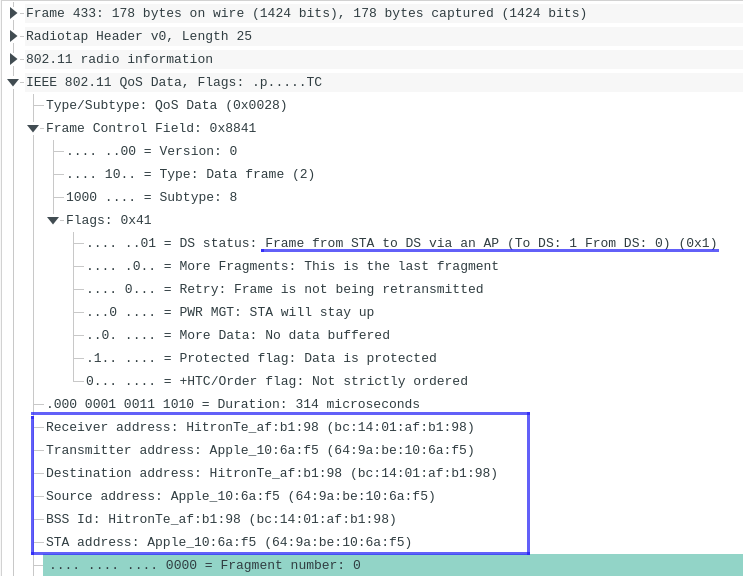
\includegraphics[width=300pt]{Prints/Questao7/questao7-433.png}
    \caption{Captura da Trama Nº 433.} \label{questao7-1-trama433}
    \end{figure}

    \par Ao analisarmos as \textit{flags} presentes no campo \textit{Frame Control}, denotamos que os valores de \textit{To} DS e \textit{From DS} são, respetivamente, 1 e 0, ou seja, contrariamente à trama analisada anteriormente, esta é direcionada ao AP tendo como origem o STA. Para além disto, poderíamos chegar à mesma conclusão a partir da análise dos endereços MAC presentes na trama: \textit{receiver} ((\textbf{bc:14:01:af:b1:98})), \textit{transmitter} (\textbf{64:9a:be:10:6a:f5}) e \textit{destination} (\textbf{bc:14:01:af:b1:98}).







\subsubsection{Que subtipo de tramas de controlo são transmitidas ao longo da transferência de dados acima mencionada? Tente explicar porque razão têm de existir (contrariamente ao que acontece numa rede Ethernet.)}

    \par Ao longo de uma transferência de dados são transmitidas tramas de controlo do subtipo \textit{Request To Send} e \textit{Clear To Send}. Estas tramas têm como objetivo evitar colisões e controlar a transmissão de dados pelo meio, uma vez que vários dispositivos podem estar ligados a um AP e, caso transmitam simultaneamente, vão existir colisões e como consequência a corrupção de pacotes.
    
    \par Assim, podemos resumir o comportamento destas tramas de controlo da seguinte forma: o STA envia tramas com pedidos de conexão (RTS) para o AP, respondendo o AP, em \textit{broadcast}, uma trama CTS. A trama CTS é "ouvida"\xspace por todos os nós, permitindo ao STA enviar os dados ao AP sem interrupções.

    \par Contrariamente, nas redes \textit{Ethernet}, este sistema não é implementado, pois estas utilizam dispositivos como \textit{switches} e \textit{hubs} que conseguem redirecionar e distribuir o tráfego na rede, em particular, na utilização de \textit{switches}, cada dispositivo tem um canal de transmissão único e direto, permitindo assim evitar colisões.





\vspace{10pt}
\subsubsection{O uso de tramas \textit{Request To Send} e \textit{Clear To Send}, apesar de opcional, é comum para efetuar "pré-reserva" do acesso ao meio quando se pretende enviar tramas de dados, com o intuito de reduzir o número de colisões resultante maioritariamente de STAs escondidas. Para o exemplo acima, verifique se está a ser usada a opção RTS/CTS na troca de dados entre a STA e o AP/Router da WLAN, identificando a direccionalidade das tramas e os sistemas envolvidos. Dê um exemplo de uma transferência de dados em que é usada a opção RTC/CTS e um outro em que não é usada}

    \par Para verificarmos se existiu algum controlo de colisões através das tramas RTS e CTS, começamos por analisar as tramas capturadas nos instantes imediatamente antes e depois da trama nº 433. Desta forma, obtivemos as seguintes tramas, não obtendo quaisquer tramas de controlo de colisões:
    
    \begin{figure}[H]
    \centering
    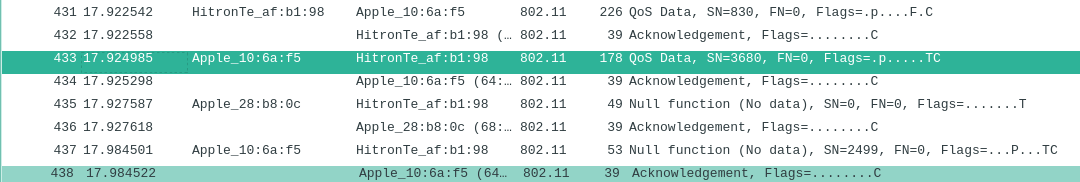
\includegraphics[width=500pt]{Prints/Questao7/questao7-Ultima.png}
    \caption{Tramas capturadas na envolvência da trama nº433.} \label{questao7-redor}
    \end{figure}
    
    \par Assim, para encontrarmos uma transferência de dados que utilize este controlo e de modo a facilitar a sua pesquisa no ficheiro de captura, desenvolvemos o seguinte filtro que irá filtrar todas as tramas RTS e CTS assim como todas as tramas de dados, tendo retirado, novamente, os valores dos subtipos do anexo dos docentes.
    
    \vspace{20pt}
    \begin{minipage}{\linewidth}
        \centering
        \fbox{
        \parbox{390pt}{
		    (wlan.fc.type\_subtype $==$ 0x1b) \textbf{or} (wlan.fc.type\_subtype $==$ 0x1c)
		    \textbf{or} 
		    \par
		    (wlan.fc.type\_subtype $>$= 0x20 \textbf{and} wlan.fc.type\_subtype $<$= 0x2f) 
        }
    }
    \end{minipage}
    
    
    \vspace{10pt}
    \par Após a aplicação do filtro, o \textit{Wireshark} apresentou várias tramas que obedeciam ao mesmo, tendo o grupo captado duas transmissões de dados que diferem na sua direcionalidade, ou seja, uma com a comunicação no sentido AP -$>$ STA e outra no sentido STA -$>$ AP.
    
    \begin{figure}[H]
    \centering
    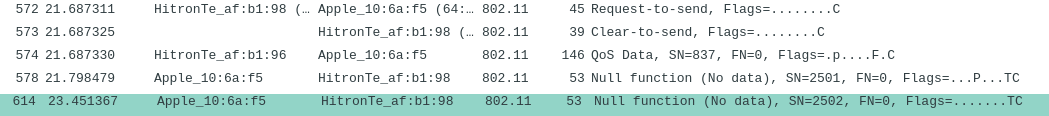
\includegraphics[width=500pt]{Prints/Questao7/questao7-AP2STA.png}
    \caption{Conjunto de tramas no sentido AP -$>$ STA.} \label{questao7-ap2sta}
    \end{figure}
    
    \begin{figure}[H]
    \centering
    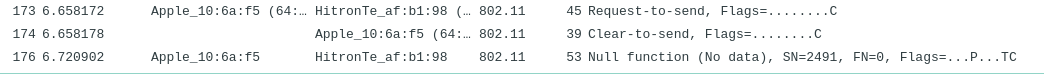
\includegraphics[width=500pt]{Prints/Questao7/questao7-STA2AP.png}
    \caption{Conjunto de tramas no sentido STA -$>$ AP.} \label{questao7-sta2ap}
    \end{figure}
    
    \par Como podemos verificar pelas Figuras \ref{questao7-ap2sta} e \ref{questao7-sta2ap}, o dispositivo de origem envia uma trama RTS ao dispostivo destino e, depois de aceite, através do envio de uma segunda trama (CTS), trocam dados entre si assim como tramas de confirmação (\textit{Acknowledgement}).